% In this section, we present our algorithm for computing the upper bound for a program $c$'s adaptivity
% $A(c)$ defined~\ref{def:trace_adapt} through static program analysis.
% This section presents the key definitions
% for the static analysis algorithm in Section~\ref{sec:algorithm-keys} before going into the detail of the algorithm,
% then shows the complete static analysis algorithm.
% \mg{
% In this section, we present our static program analysis for computing an upper bound on the adaptivity a program $c$
% }
In this section, we present our static program analysis for computing an upper bound on the 
execution-based reachability times for every label $l$ of an arbitrary program $c$.
% , as defined in last section.
%
\subsection{Algorithm Overview}
\label{sec:alg_overview}
In order to have the upper bound of the reachability for every label of a program $c$, we design 
a path sensitive reachability bound analysis algorithm {\THESYSTEM}.
It can be summarized as the following steps: 
% \begin{figure}
%   \centering    
% 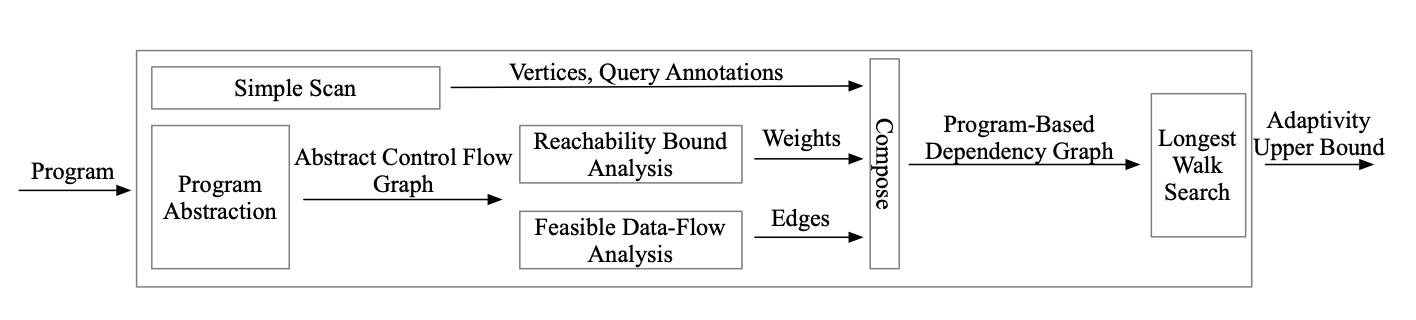
\includegraphics[width=1.0\columnwidth]{adapfun.png}
%   \vspace{-0.3cm}
%   \caption{The overview of {\THESYSTEM}}
%   \label{fig:adaptfun}
%   \vspace{-0.5cm}
% \end{figure}
%
%
\begin{enumerate}
\item  In Section~\ref{sec:abscfg}, we first construct an abstract control flow graph based on $c$, by computing an abstract transition 
for every labeled command. 
This graph is used in Section~\ref{sec:reachabilitybound_algorithm} for analyzing program's reachability bound.
% see Section~\ref{sec:alg_vertexgen}
\item The Section~\ref{sec:reachabilitybound_algorithm} computes program's reachability bound in two steps as follows.
\begin{enumerate}
\item The Section~\ref{sec:pathinsensitive_rb} estimates path-insensitive reachability upper bound for every while loop command in $c$.
% Vertices are the assigned variables with unique labels, which is extracted directly from the program, 
% Every vertex come with a weight, which tells the maximal times each vertex and edge can be visited in realistic execution. This weight is estimated by a reachability bound analysis on each vertex, See Section~\ref{sec:alg_weightgen}.
% \item Each edge also vertices considers both control flow and data flow, See
% Section~\ref{sec:alg_edgegen}
\item The Section~\ref{sec:pathsensitive_rb} estimates the path-sensitive reachability upper bound 
for every program locations (i.e., every command label) through four steps:
\begin{enumerate}
\item {\THESYSTEM} firstly refines this program into the rephrased and refined program, based on the abstract control flow graph
generated in Section~\ref{sec:abscfg}.
\item Then in the second and third steps, it performs the Outside-In and Inside-Out Algorithms 
on this refined program, and obtains 
path-sensitive reachability bound for each edge on the abstract control flow graph.
\item At the last step, {\THESYSTEM} computes the path-sensitive reachability bound for every label in this program $c$ by summarizing 
the path-sensitive reachability bound of each edge on the abstract control flow graph.
\end{enumerate}
\end{enumerate}
% Finally, with all the ingredients ready, we construct the final approximated program-based dependency graph in Section~\ref{sec:alg_graphgen}
\end{enumerate}

% the algorithm  without extra static analysis technique.
% \\
% Overall, this program-based graph has a similar topology structure as 
% % the one
% % of 
% the Execution-Based Dependency Graph. It has the same
% vertices and query annotations, but approximated edges and weights. We call the graph generated by static analysis techniques, static analysis dedendency graph. 
% \item Then in the last phase in Section~\ref{sec:alg_adaptcompute}, $\THESYSTEM$
% % we compute the upper bound for adaptivity over this approximated graph:
% % , as an upper bound for
% % program's adaptivity
% computes the upper bound for adaptivity over this approximated graph.
% in the last phase of this algorithm in Section~\ref{sec:alg_adaptcompute}.
% \subsection{Adaptivity Based on Program Analysis in \THESYSTEM}
% In order to give a bound on the program's adaptivity, we first build a
% program-based data-dependency graph to {over-}approximate the
% trace-based dependency graph.  Then, we define a program-based
% adaptivity over this approximated graph, as an upper bound for
% $A(c)$.
% %
% \subsection{ $\THESYSTEM$ Analysis Algorithm}
% \subsection{Dependency Graph Estimation}
% \subsection{Vertices Estimationn}
% \label{sec:alg_vertexgen}
% The first component of every vertex in the static analysis dependency graph are actually identical as the  Execution-Based Dependency Graph, which are assigned variables in the program annotated with the unique label(line number). 
% These vertices are collected by statically scanning the program, like what we do for vertices of its Execution-Based Dependency Graph. 
% The vertices are defined formally as follows.

%   \highlight{
% \[
%     \progV^0(c) \triangleq \left\{ 
%   (x^l, w) \in \mathcal{LV} \times \mathcal{A}_{\lin}
%   ~ \middle\vert ~
%   x^l \in \lvar(c)
%   \right\}
%   \]
%   }
%   %
% where $\mathcal{A}_{\lin}$ is the set of arithmetic expressions over $\mathbb{N}$ and program's input variables. 
% The weight $w$ for every vertex will be computed in following step in Section~\ref{sec:alg_weightgen}.
% The static scanning of the programs also tells us whether one vertice(assigned variable) is assigned by a query request. We have similar definition when defining the Execution-Based Dependency Graph, 
% a set of pairs $\progF(c) \in \mathcal{P}(\mathcal{LV} \times \{0, 1\} )$ 
% % is the set of pairs 
% % The weight for each vertex in $\progV(c)$ is computed 
% mapping each $x^l \in \progV(c)$ to a flag, either $0$ or $1$, where $1$  means $x^{l}$ is a member of $ \qvar_{c}$, a set of those variables assigned with query requests, and $0$ means $x^{l}$ not in this set. It is defined formally below.

% \[\progF(c) =\left\{(x^l, n)  \in  \mathcal{LV} \times \{0, 1\} 
% ~ \middle\vert ~
% x^l \in \lvar_{c},
% n = 1 \iff x^l \in \qvar_{c} \land n = 0 \iff  x^l \not\in \qvar_{c} .
% \right\}\]
%

% \wq{To do: Add $\THESYSTEM$, a data flow analysis algorithm to scan the program and give a graph.}
% {\THESYSTEM} consists of three phases: 
% \begin{enumerate}
%     \item Generating an abstract control flow graph with each edge representing an abstract event transiting between two command labels. 
%     \item Computing the value bound invariant for each variable in the event and 
%     the event transition closure over the abstract control flow graph,
%     we get the reachability bound for each labeled command.
%     \item Refining the abstract control flow graph with data-flow, by performing the reaching definition analysis, we generate a weighted data control flow graph.
%     \item An algorithm to find the appropriate path in the weighted data control flow graph
% \end{enumerate}

% \begin{enumerate}
%     \item An algorithm to generate a precise data control flow graph
%     \item An algorithm to perform a Reachability number analysis to calculate the weight of each node in the graph generated in phase 1.
%     \item An algorithm to find the appropriate path in the weighted data control flow graph
% \end{enumerate}

% \subsection{Edge and Weight Estimation}
% \label{sec:alg_weightedgegen}

% Since the edges of the execution-based graph of a program relies on the dependency relation, which handles both control flow and data flow, as an over-approximation of this graph, the edges of our static anlaysis dependency graph also covers these two kind of flows. We develop a feasible data flow relation to catch these two flows, in Section~\ref{sec:alg_edgegen}.


% The weight of every vertice in the execution-based graph is built on all possible execution traces.
% In order to over-approximate the weight statically but still tightly, we present a symbolic reachability bound analysis for estimation of the weight of each vertice(label) in Section~\ref{sec:alg_weightgen},
% in spirit of some reachablility bound techiniques.


% The edges and weight estimation are both performed on basis of an abstract control flow graph of the program, we first show how to generate this abstract execution control flow graph before the introduction of  the edge and weight estimation.  

% This analysis first 
%  generate an abstract control flow graph
%  over all program labels, 
% in order to analyzing the data flow relations through variables assigned in every labeled command,
% and the reaching time of each variable.
% Then, it refines this control flow graph 
% % into a weighted data-dependency graph, 
% and generate the Program-Based Dependency Graph,
% through the data flow and reaching bound analysis results.
% In the last step, it finds the longest finite walk in this weighted data control flow graph w.r.t. the query variables,
% and return the number of query vertices traversed alongside.
% % \wq{To do: Add $\THESYSTEM$, a data flow analysis algorithm to scan the program and give a graph.}
% To be more specific, {\THESYSTEM} consists of five phases as follows,
% \\
% % \jl{Better to have a graph or picture of overview of the algorithm}
% \todo{graph}
% \todo{pass again}
% This analysis
% \begin{enumerate}
%     % \item Generating 
%     \item first generate 
%     an abstract control flow graph
%     %  over all labels,
%     (remove?? with program's labels as vertices and abstract transitions as edges)
%     in Section~\ref{sec:abscfg},
%     % used to analyze 
%     for analyzing the weight of every vertex in $\progV(c)$ and edges between every vertex in $\progV(c)$ in the next two steps;
%     %  \ref{sec:alg_weightgen} and 
%     % \ref{sec:alg_edgegen}.

%     % which are used as program's control locations,
%     %
%     \item then use the abstract control flow graph generated above, 
%     compute the weight of every vertex in $\progV(c)$ by computing a symbolic reachability bound for each label in Section~\ref{sec:alg_weightgen},
%     % \\
%     \item and then use the same graph again to estimate the edges between every vertex in $\progV(c)$ by computing the feasible data flow relation between every labeled variables in Section~\ref{sec:alg_edgegen}.
  
% \end{enumerate}

\subsection{Abstract Execution Control Flow graph}
\label{sec:abscfg}

This estimation is performed on basis of an abstract control flow graph of the program, 
we first show how to generate this abstract execution control flow graph before the introduction of  the edge and weight estimation.  
We discuss the vertices and edge of the
abstract control flow graph for a program $c$, $\absG(c)$.

\subsubsection{Vertices Construction}
\label{sec:abscfg-vertex}
Every 
vertex corresponds to the unique
label.
Specifically,
the vertices of this graph is the set of $c$'s labels with the exit label ${\lex}$, 
\[ 
  \absV(c) = \lvar(c)\cup\{{\lex}\}
  \]
%  corresponding to a label command in the program.

\subsubsection{Edge Construction}
\label{sec:abscfg-edge}
  The edge in the abstract control flow graph comes from the abstract execution trace of the program. 
  The abstract execution trace, an abstract representation of the execution, consists of a list of abstract transitions. 
  Then, every abstract transition in the abstraction execution trace corresponds to an edge in the abstract control flow graph. In another word, the edge $(l_1, dc, l_2)$ in the abstract control flow graph, represents an abstract transition 
 from $l_1$ to $l_2$, with a set of difference constraints $dc$. 
 Also notice, the difference constraints generated during the abstract transition appears in the edge as annotation.

  Overall, the vertices can be easily collected and the key point of construction of the abstract execution control flow graph for a program is the abstract execution trace, 
  which relies on the abstraction of expression and abstract transition (we also call it abstract event), we will discuss in the following section.
   To make it easy to understand, abstract control flow graph is a control flow graph, with difference constraints on every edge.

%
\paragraph*{Expression Abstraction}

The expression assigned to the variable on the left hand of the assignment command is abstracted to an abstract value: (adopted from the expression abstraction method in paper \cite{sinn2017complexity}). The abstract value is expressed in the form of Difference constraint, denotated as $DC : \mathcal{VAR} \cup \constdom \to \mathcal{\mathcal{VAR} \times (\mathcal{VAR} \cup \constdom) } \times (\mathbb{Z} \cup \{\infty\})$.  $\constdom$ is called the Symbolic Constant defined as $\constdom \triangleq \mathbb{N} \cup \inpvar$
%  \cup \{\max{(\dbdom)}\} $, 
which consists of 
natural numbers $\mathbb{N}$,
the program's input variables $\inpvar$. 
% and a constant value $Q_m$ for estimating the upper bound of variables which are
% assigned by queries. 

Give an instance of difference constraint used here,
$DC(\mathcal{VAR}  \cup \constdom) \cup \{\top\}$ represents all the difference constraints over 
variable and symbolic constants. 
% The difference constraint $DC$ over $\mathcal{VAR} \cup \constdom$ 
It is a set of the inequality of form $x \leq y + v$ where $x \in \mathcal{VAR} $, 
$y \in \mathcal{VAR}  \cup \constdom$ and $v \in \mathbb{Z}$. 
This difference constraint is defined in the same way as
\cite{sinn2017complexity}. For concise, we use $\dcdom^{\top}$ to represent the $DC(\mathcal{VAR}  \cup \constdom) \cup \{\top\} \cup \mathcal{BEXPR}$.

We show the expression abstraction $\absexpr : \expr \to \mathcal{VAR} \to \dcdom^{\top} $ below.

% We introduce the following notations and operations first
% % an expression abstraction method based on the expression abstraction in paper \cite{sinn2017complexity}.
% \\
% % is enriched into $\constdom \triangleq \mathbb{N} \cup \inpvar \cup \{\max{(\dbdom)}\} $.
% T
% \\

% represents the set of inequality over all $\mathcal{VAR}  \cup \constdom$. 

% The symbolic constant is enriched into $\constdom \triangleq \mathbb{N} \cup \inpvar \cup \{\max{(\dbdom)}\} $.
% It consists of 
% natural number $\mathbb{N}$,
% the symbolic constants $\inpvar$ (i.e., the set of the program's input variables), 
% and a constant value $Q_m$ for estimating the upper bound of variables which are
% assigned by queries.
% \\
% The symbolic constant is enriched into $\constdom \triangleq \mathbb{N} \cup \inpvar \cup \{\max{(\dbdom)}\} $.
% \\

% % $ \absdom: \mathcal{P}(DC(\mathcal{VAR}  \cup \constdom) \cup \{\top \})$:
% \\
% $\constdom: \mathbb{N} \cup \inpvar \cup \{\max{(\dbdom)}\} $ 
% The  constant 
% \\
% % $DC(\mathcal{VAR}  \cup \constdom)$ represents the set of inequality over all $\mathcal{VAR}  \cup \constdom$.
% \\

% \[
%   \begin{array}{ll} 
%     \absexpr(y + c, x)  = x' \leq y + c  & c \in \mathbb{N} \land y \in (VAR \cup \constdom) \\
%     \absexpr(y - c, x)  = x' \leq y - c  & c \in \mathbb{N} \land y \in (VAR \cup \constdom) \\
%     \absexpr(v, x)  = x' \leq v + 0  & v \in (VAR \cup \constdom) \\
%     \absexpr(\aexpr, x) = x' \leq 0 + \infty   & \aexpr \text{ doesn't have any of the forms as above} \\
%     \absexpr(\qexpr, x)  = x' \leq 0 + Q_m & \qexpr \text{ is a query expression}  \\
%     \absexpr(\bexpr, x) = x' \leq 0 + 1   & \bexpr \text{ is a boolean expression} \\
%   \end{array}
%   \]
  \[
    \begin{array}{ll} 
      \absexpr(x - v, x)  = x' \leq x - v  & x \in \grdvar \land v \in \mathbb{N} \\
      \absexpr(y + v, x)  = x' \leq y + v  & x \in \grdvar \land v \in \mathbb{Z} \land y \in (\grdvar \cup \constdom) \\
      \absexpr(v, x)  = x' \leq v + 0  & x \in \grdvar \land v \in (\grdvar \cup \constdom) \\
      \absexpr(y + v, x)  = x' \leq y + v & \\
      \grdvar = \grdvar \cup \{y\} & x \in \grdvar \land v \in \mathbb{Z} \land y \notin (\grdvar \cup \constdom)  \\
      % \absexpr(\qexpr, x)  = x' \leq 0 + Q_m & x \in \grdvar \land \qexpr \text{ is a query expression}  \\
      \absexpr(\bexpr, \top) = \bexpr   & \\
      % \absexpr(y + v, x)  = x' \leq y + v & \\
      \grdvar = \grdvar \cup FV(\bexpr) &  x \in \grdvar \land \bexpr \text{ is a boolean expression} \\
      \absexpr(\expr, x) = x' \leq \infty  &  x \in \grdvar \land \expr \text{ doesn't have any of the forms as above} \\
      \absexpr(\expr, x) = \top  &  x \notin \grdvar \\
    \end{array}
    \]
  
  % \wq{ 
    $\grdvar$ is the set of variables used in the guard expression of every while command in the program $c$. 
  % }. 
  In the case 4, if a variable $x$, belonging to the set 
  $\grdvar$ is updated by a variable $y$, which isn't in this set, 
  we add $y$ into the set $\grdvar$ and repeat 
  above procedure  until $\grdvar$ and $\absexpr(\expr, x)$ is stabilized. 
  % \wq{I do not understand this sentence:-(}
  \\
Specifically 
% understanding the intuition, 
we handle a 
% simplified 
normalized guard expression ($ x > 0$ for $x^l \in \lvar_c$)
 in $\ewhile$, and 
%  \wq{I do not understand this sentence:-(}
%  .
% \\
% The counter variables only increase, decrease or reset by expression in the form of arithmetic minus and plus (able to extend to max and min.)
the counter variables only increase, decrease or reset by 
% expression in the form of 
simple arithmetic expression (mainly multiplication, division, minus and plus (able to extend to max and min)). 
This is the same as in paper \cite{sinn2017complexity}. 
\\
For more complex expression assignments, where the counter reset, or calculated from $\elog$, 
multiplication or division, and expressions involving multiple variables, the constraint is approximated as reset of $\infty$.
\\
% This simplification \wq{which part we simplify here?} 
This approximation strategy
doesn't affect our analysis results in our examples. It is easy to extend the normalized expression 
into more complex forms as in \cite{sinn2017complexity}, as well as the 
counter variable manipulation with more advanced expressions.
% \\ 
% The boolean expression in the guard of $\ewhile$ command is normalized into form of $ x > 0$ where $x^l \in \lvar_c$ for some $l$.


\paragraph{Abstract Initial and Final State}
%
Abstract initial state: $\absinit(c) \in \ldom$,
Abstract Final State: $\absfinal(c) \in \mathcal{P}(\ldom \times \dcdom^{\top})$

The \emph{Abstract initial state} for a program $c$ is the initial label of this program.
This label corresponds to the first labeled command of this program 
when executing this program.
\\
Given a program $c$, its abstract initial state is computed as follows,
%
\[
  \begin{array}{ll}
    \absinit(\clabel{\assign{x}{\expr}}{}^l)  & = l  \\
    \absinit(\clabel{\assign{x}{\expr}}{}^l)  & = l \\
    \absinit(\clabel{\eskip}^{l})  & = l \\
    \absinit(\eif [b]^l \ethen c_1 \eelse c_2)  & = l \\
    \absinit(\ewhile [b]^l \edo c)  & = l \\
    \absinit(c_1 ; c_2)  & = \absinit(c_1) \\
 \end{array}
 \]
%

The \emph{Abstract Final State} of the program $c$, 
$\absfinal(c) \in \mathcal{P}(\ldom \times \dcdom^{\top})$
is a set of pairs, with a label as first component and a constraint as the second component.
Every pair in $\absfinal(c)$ corresponds to a labeled command of $c$,
and the constraint in this pair is computed by $\absexpr$ in the first step.
\\
Given a program $c$, its final state is computed as follows,
$\absfinal: \cdom \to \mathcal{P}(\ldom \times \dcdom^{\top})$,
% computes the set of Abstract Final State for the command. 
 \[
  \begin{array}{ll}
    \absfinal(\clabel{\assign{x}{\expr}}{}^l)  & = \{(l, \absexpr\eapp (\expr, x))\}  \\
    %  \absfinal(\clabel{\assign{x}{\query(\qexpr)}}{}^l)  & = \{
    %   (l, x' \leq 0 + Q_m )\}  \\
     \absfinal(\clabel{\eskip}^{l})  
     & = \{(l, \top)\} \\
     \absfinal(\eif [b]^l \ethen c_1 \eelse c_2)  & = \absfinal(c_1) \cup \absfinal(c_2) \\
     \absfinal(\ewhile [b]^l \edo c)  & = \{(l, \absexpr(\bexpr, \top))\} \\
     \absfinal(c_1 ; c_2)  & =  \absfinal(c_2) \\
 \end{array}
 \]
 %
 \paragraph{Abstract Event and Execution Trace} 
 \emph{Abstract Event}: 
   $\absevent \in $
   $\ldom \times \dcdom^{\top} \times \ldom$,
   \emph{Abstract Execution Trace}: $\absflow \in \cdom \to \mathcal{P}( \ldom \times \dcdom^{\top} \times \ldom )$

 The abstract event is generated during computing its abstract execution trace, its type is defined as follows,
 \begin{defn}[Abstract Event]
   \label{def:abs_event}
   Abstract Event: 
   $\absevent \in $
   $\ldom \times \dcdom^{\top} \times \ldom$
   is a 
   % pair of abstract initial state and final state.
   triple where the first and third components are labels,
   second component is a constraint from $\dcdom^{\top}$.
   % the thrid % computed from program's abstract final and initial state, $\absfinal(c)$ and $\absinit(c)$ with formal definition, and algorithm detail in Appendix.
   %  the constraint and the third corresponds to a final state.
   \end{defn}
   Specifically, in an abstract event, 
   the first label correspond to an initial state, and 
   the second label and the constraint correspond to an abstract final state.
  The abstract initial state is a label from $\ldom$.
 The abstract final state is a pair from $\ldom \times \dcdom^{\top}$,  
 where first component is a label from $\ldom$ and the second component is a constraint from $\dcdom^{\top}$.
 %
 For simplicity, we use $\mathcal{P}(\absevent)$ represent the power set of all abstract events, and we have $\absflow(c) \in \mathcal{P}(\absevent)$.

%  Now, we  extract the abstract execution trace  $\absflow(c)$ for a program, which computes the 
 The \emph{Abstract Execution Trace} for program $c$ is a set of the abstract events $\absevent$.
 Its type is formally defined as follows in Definition~\ref{def:abs_trace}.
 %
 \begin{defn}[Abstract Execution Trace]
 \label{def:abs_trace}
  $\absflow \in \cdom \to \mathcal{P}( \ldom \times \dcdom^{\top} \times \ldom )$
  \end{defn}
 %
 The \emph{Abstract Execution Trace} for program $c$ is computed as follows.
 \\
  % We now show how to compute the abstract execution trace. 
 We first append a $\eskip$ command with 
%  a symbolic label $l_e$, i.e., $\clabel{\eskip}^{l_e}$ at the end of the program $c$, and compute the $\absflow(c) = \absflow'(c')$ for $c'$, where $c' = c;\clabel{\eskip}^{l_e}$ as follows,
the label $\lex$, i.e., $\clabel{\eskip}^{l_{ex}}$ at the end of the program $c$, and construct 
the program $c' = c;\clabel{\eskip}^{l_{ex}}$.
Then, we compute the $\absflow(c) = \absflow'(c')$ for $c'$ as follows,
 %
 {\footnotesize
 \[
   \begin{array}{ll}
      \absflow'(\clabel{\assign{x}{\expr}}{}^l)  & = \emptyset  \\
      \absflow'(\clabel{\assign{x}{\query(\qexpr)}}{}^l)  & = \emptyset  \\
      \absflow'([\eskip]^{l})  & = \emptyset \\
      \absflow'(\eif [b]^l \ethen c_t \eelse c_f)  & =  \absflow'(c_t) \cup \absflow'(c_f)
        \\ & \quad 
        \cup \{(l, \absexpr(\bexpr, \top),  \absinit(c_t) ) ,  (l, \absexpr(\neg\bexpr, \top), \absinit(c_f)) \} \\
       \absflow'(\ewhile [b]^l \edo c_w)  & =  \absflow'(c_w) \cup \{(l, \absexpr(\bexpr, \top), \absinit(c_w)) \} 
       \\ & \quad 
       \cup \{(l', dc, l)| (l', dc) \in \absfinal(c_w) \} \\
       \absflow'(c_1 ; c_2)  & = \absflow'(c_1) \cup  \absflow'(c_2) 
       \\ & \quad 
       \cup \{ (l, dc, \absinit(c_2)) | (l, dc) \in \absfinal(c_1) \} \\
   \end{array}
   \]
   }

   Notice $\absflow'([x := \expr]^{l})$, $\absflow'([x := \query(\qexpr)]^{l})$ and $\absflow'([\eskip]^{l})$ are all empty set. 
   For every event $\event$ with label $l$ in an execution trace $\trace$ of program $c$, 
   there is an abstract event in program's abstract execution trace of form $(l, \_, \_)$.  
   We also show the soundness of the abstract execution trace in Appendix.
  %  which says 
  %  \wq{...}
   \begin{lem}[Soundness of the Abstract Execution Trace]
     \label{lem:abscfg_sound}
   Given a program ${c}$, we have:
   %
   \[
     \begin{array}{l}
       \forall \vtrace_0, \trace \in \mathcal{T} ,  \event = (\_, l, \_) \in \eventset \st
   \config{{c}, \trace_0} \to^{*} \config{\eskip, \trace_0 \tracecat \vtrace} 
   \land \event \in \trace 
   \\
   \qquad \implies \exists \absevent = (l, \_, \_) \in (\ldom\times \dcdom^{\top} \times \ldom) \st 
   \absevent \in \absflow(c)
   \end{array}
   \]
   \end{lem}
%    This lemma is proved formally in Appendix~\ref{apdx:pathinsensitive_rb_soundness}.
% For every event $\event$ with label $l$ in an execution trace $\trace$ of program $c$, 
% there is an abstract event in program's abstract execution trace of form $(l, \_, \_)$. 
This lemma is proved formally in Lemma~\ref{lem:abscfg_sound} in Appendix~\ref{apdx:pathinsensitive_rb_soundness}.
\\
For every labeled variable in program $c$, $x^l \in \lvar_c$, 
there is a unique abstract event in program's abstract execution trace $\absevent \in \absflow(c)$ of form $(l, \_, \_)$. 
\begin{lem}[Uniqueness of the Abstract Execution Trace]
  \label{lem:abscfg_unique}
Given a program ${c}$, we have:
%
\[
  \begin{array}{l}
    \forall \vtrace_0, \trace \in \mathcal{T} ,  \event = (\_, l, \_, \_) \in \eventset^{\asn} \st
\config{{c}, \trace_0} \to^{*} \config{\eskip, \trace_0 \tracecat \vtrace} 
\land \event \in \trace 
\\
\qquad \implies \exists! \absevent = (l, \_, \_) \in (\ldom\times \dcdom^{\top} \times \ldom) \st 
\absevent \in \absflow(c)
\end{array}
\]
\end{lem}
This lemma and proof is also 
formalized in Lemma~\ref{lem:absevent_unique} in Appendix~\ref{apdx:pathinsensitive_rb_soundness}.

Then, we build the edge for $c$'s abstract control flow graph as follos,
\[
  \absE(c) = \{(l_1, dc, l_2) | (l_1, dc, l_2) \in \absflow(c)\}
  \]

% We have a pre-processing algorithm to go through the programs and returns the list of labels associating with a loop and whose visiting times need to be analyzed.
%
\paragraph{Abstract Control Flow Graph} 
With the vertices $\absV(c)$ and edges $\absE(c)$ ready, we construct the abstract control flow graph, formally 
% Through a program $c$'s abstract execution trace, its abstract control flow graph is computed 
defined in 
Definition~\ref{def:abs_cfg}.
%
\begin{defn}[Abstract Control Flow Graph]
\label{def:abs_cfg}
Given a program $c$, 
with its abstract control flow $\absflow(c)$
its abstract control flow graph $\absG(c) =(\absV(c), \absE(c), \absW(c))$ is defined as follows,
\\
$\absE(c) = \{(l_1, dc, l_2) | (l_1, dc, l_2) \in \absflow(c)\}$,
\\
$\absV(c) = \lvar(c)\cup\{l_{ex}\}$
\\
 $\absW(c) 
\triangleq \left\{ (l, w) \in \mathbb{L} \times EXPR(\constdom) \right\}$.
\end{defn}
% \\
Notice we also define the $\absW(c)$ in this graph without giving an actual value.
This $\absW(c)$ is the set of weight for every 
% vertex 
label. The weight $w \in EXPR(\constdom)$ is a symbolic expression over the symbolic constant, 
which is the estimated upper bound on the number of visiting time for every control location
through the reachability bound analysis as follows.
%
$EXPR(\constdom)$ is the set of all the symbolic expressions 
over $\constdom$, which is a subset of arithmetic expressions over $\mathbb{N}$ with input variables.
For concise, $\mathcal{A}_{\lin}$ is used as the same meaning of $EXPR(\constdom)$ in the follows, to denote the arithmetic expression 
over the symbolic variables, (i.e., $\mathbb{N}$ with input variables).
\subsubsection{Abstract Control Flow Graph through an Example}
\label{sec:abscfg_example}
% 
% Look at the two-round example again, its generated abstract control is shown as in Figure~\ref{fig:adapfun_tworound}(a).
% In this abstract control flow graph, every vertex is a label,
% corresponding to a label command in the program.
% Each directed 
% edge represents an abstract transition 
% between two control locations, 
% i.e., the labels of two commands (we call the labels also control location and they refer to the same thing), 
% where the second labeled command will be executed after execution of the command with first label.
% For example, the edge $0, a \leq 0, 1$ on the top, represents,
% from location $0$, the command 
% $\clabel{\assign{a}{0}}^0$ is executed with next continuation location $1$,
% where the 
% command $\clabel{\assign{j}{k}}^1$ will be executed next.
% The constraint $a \leq 0$ is generated by abstracting from the assignment command $\assign{a}{0}$,
% representing that value of $a$ is less than or equals to $0$ after 
% location $0$ before executing command at line $1$.
% %
% The same way for the rest edges' constructions.
%
\begin{example}[The Abstract Control Flow Graph for A Simple While Loop Program]
  \label{ex:whileSim_abscfg}
    For the simple while loop example program, 
its abstract control flow graph is shown as in Figure~\ref{fig:whileSim_abscfg}(b).
For example, the edge $(0, a' \leq 0, 1)$ on the top, tells us the command 
$\clabel{\assign{a}{0}}^0$ is executed with next continuation point $1$,
where the 
command $\clabel{\assign{j}{k}}^1$ will be executed next.
The constraint $a' \leq 0$ is a difference constraint, generated by abstracting from the assignment command $\assign{a}{0}$.
It represents that the value of $a$ is less than or equals to $0$ after 
execution of $\clabel{\assign{a}{0}}^0$ and before executing $\clabel{\assign{j}{k}}^1$.
The difference constraint is an inequality relation, 
the left-hand side of the inequality $x'$ denotes the variable $x$
after executing the command at $l$
and the right-hand side describes the variable $x$ in the state before the execution. 
Look at the $a' < a+x $ on the edge $5$ to $2$, which describes the execution of the command at line $5$, 
which is an assignment $a' = a+x$. The $a'$ on the left side of $a' < a+x$ represents the value of $a$ after the assignment,
while the right-hand side $a$ stores the value before the assignment. 
% $top$ means there is no assignment executed, for example, 
I have 
The boolean constraint $j \leq 0 $ on the edge $2 \to 6$, 
represents the negation of the testing guard $j > 0$
in the $\ewhile$ command with loop header at line $2$.
%
% The same way for the rest edges' constructions.
\begin{figure} 
  \centering
  \begin{subfigure}{.7\textwidth}
  \begin{centering}
  {\small
  $
  \kw{whileSim(k)} \triangleq
    \begin{array}{l}
        \clabel{ \assign{a}{0}}^{0} ;   
              \clabel{\assign{j}{k} }^{1} ;\\
              \ewhile ~ \clabel{j > 0}^{2} ~ \edo ~ 
              \Big(
               \clabel{\assign{x}{j} }^{3}  ;
               \clabel{\assign{j}{j-1}}^{4} ;
              \clabel{\assign{a}{x + a}}^{5}  \Big);\\
              \clabel{\assign{l}{k * a} }^{6}
          \end{array}
  $
  }
  \caption{}
  \end{centering}
  \end{subfigure}
    \begin{subfigure}{.45\textwidth}
    \begin{centering}
  \begin{tikzpicture}[scale=\textwidth/20cm,samples=200]
  \draw[] (-7, 10) circle (0pt) node{{ $0$}};
  \draw[] (0, 10) circle (0pt) node{{ $1$}};
  \draw[] (0, 7) circle (0pt) node{\textbf{$2$}};
  \draw[] (0, 4) circle (0pt) node{{ $3$}};
  \draw[] (0, 1) circle (0pt) node{{ $4$}};
  \draw[] (-7, 1) circle (0pt) node{{ $5$}};
  % Counter Variables
  \draw[] (6, 7) circle (0pt) node {\textbf{$6$}};
  \draw[] (6, 4) circle (0pt) node {{ $\lex$}};
  %
  % Control Flow Edges:
  \draw[ thick, -latex] (-6, 10)  -- node [above] {$a' \leq 0$}(-0.5, 10);
  \draw[ thick, -latex] (0, 9.5)  -- node [left] {$j' \leq k$} (0, 7.5) ;
  \draw[ thick, -latex] (0, 6.5)  -- node [right] {$j > 0$}  (0, 4.5);
  \draw[ thick, -latex] (0, 3.5)  -- node [right] {$x' \leq j$} (0, 1.5) ;
  \draw[ thick, -latex] (-0.5, 1)  -- node [above] {$j' \leq j - 1$} (-6, 1) ;
  \draw[ thick, -latex] (-6, 1.5)  -- node [left] {$a' \leq x + a$} (-0.5, 7)  ;
  \draw[ thick, -latex] (0.5, 7)  -- node [above] {$ j \leq 0 $}  (5.5, 7);
  \draw[ thick, -latex] (6, 6.5)  -- node [right] {$l' \leq k * a$} (6, 4.5) ;
  \end{tikzpicture}
  \caption{}
    \end{centering}
    \end{subfigure}
    \begin{subfigure}{.45\textwidth}
      \begin{centering}
    %   \todo{abstract-cfg for two round}
    \begin{tikzpicture}[scale=\textwidth/20cm,samples=200]
    \draw[] (-10, 10) circle (0pt) node{{ $0: 1$}};
    \draw[] (0, 10) circle (0pt) node{{ $1: 1$}};
    \draw[] (0, 7) circle (0pt) node{\textbf{$2: k$}};
    \draw[] (0, 4) circle (0pt) node{{ $3: k$}};
    \draw[] (0, 1) circle (0pt) node{{ $4: k$}};
    \draw[] (-10, 1) circle (0pt) node{{ $5: k$}};
    % Counter Variables
    \draw[] (6, 7) circle (0pt) node {\textbf{$6: 1$}};
    \draw[] (6, 4) circle (0pt) node {{ $\lex: 1$}};
    %
    % Control Flow Edges:
  \draw[ thick, -latex] (-8, 10)  -- node [above] {$a' \leq 0$}(-1.5, 10);
  \draw[ thick, -latex] (0, 9.5)  -- node [left] {$j' \leq k$} (0, 7.5) ;
  \draw[ thick, -latex] (0, 6.5)  -- node [right] {$j > 0 $}  (0, 4.5);
  \draw[ thick, -latex] (0, 3.5)  -- node [right] {$x' \leq j$} (0, 1.5) ;
  \draw[ thick, -latex] (-1.5, 1)  -- node [above] {$j' \leq j - 1$} (-8, 1) ;
  \draw[ thick, -latex] (-8, 1.5)  -- node [left] {$a' \leq x + a$} (-1.5, 7)  ;
  \draw[ thick, -latex] (1.5, 7)  -- node [above] {$j \leq 0 $}  (4.5, 7);
  \draw[ thick, -latex] (6, 6.5)  -- node [right] {$l' \leq k * a$} (6, 4.5) ;
    \end{tikzpicture}
    \caption{}
      \end{centering}
      \end{subfigure}
    \caption{(a) The Simple While Loop Example Program $\kw{whileSim(k)}$
    (b) The abstract control flow graph for $\kw{whileSim(k)}$  
    (c) The abstract control flow graph with the path insensitive reachability bound for $\kw{whileSim(k)}$.}
    \label{fig:whileSim_abscfg}
  \end{figure}
\end{example}
%
\subsection{\highlight{Reachability Bound Analysis}}
\label{sec:reachabilitybound_algorithm}
%
% In order to estimate weight for every vertex in $\progV(c)$,
%  we first show how to compute the reachability bound for every label in $c$
%  % (i.e., every vertex in $\absV(c)$)
%  (i.e., the $\absW(c)$), 
%  then show how to compute the weight for every vertex in $\progV(c)$.
%  \\
%  Through the edges in $\absG(c)$, which correspond to $c$'s abstract transition between labels,
%  \wq{In order to estimate weight for every vertex in the static analysis dependency graph($\progV(c)$), we want to find out the upper bound on 
%  the number of times the labeled command (uniquely associated with a vertex in $\progV(c)$) may be executed when running the program.
%  This information can be obtained by computing the reachability bound for every vertice in the abstract control flow graph ($\absW(c)$), because
%  the vertices in the two graph share the same unique label, the line number. We can easily show that the reachability bound on one vertex of the actract control flow graph is also the upper bound for the corresponding vertex in the static analysis dependency graph, both vertices share the same unique line number.}
%  We perform the symbolic reachability bound anaysis on the abstract control flow graph, 
%  through the edges in $\absG(c)$, which correspond to $c$'s abstract transition between labels.
%  we infer the invariant for every variable, and compute the transition closure for every abstract transition. By solving the closure
%  with the invariants of variables involved in this closure for every transition, we compute
%  the symbolic reachability bound of every commands corresponding to this transition.
%  \\
%  Specifically in four steps, Variable Modification Tracking, Local Bounds Computation,
%  the symbolic reachability bound of every commands corresponding to this transition. Specifically, this analysis can be performed in four steps:
%   Variable Modification Tracking, Local Bounds Computation,
%  Invariant Inference and Closure Generation, and Reachability Bound Computation,
% {In order to estimate weight for every vertex in the static analysis dependency graph($\progV(c)$), we want to find out the upper bound on 
% the number of times the labeled command (uniquely associated with a vertex in $\progV(c)$) may be executed when running the program.
% This information can be obtained by computing the reachability bound for every vertex in the abstract control flow graph ($\absW(c)$), because
% the vertices in the two graph share the same unique label, the line number. We can easily show that the reachability bound on one vertex of the abstract control flow graph is also the upper bound for the corresponding vertex in the static analysis dependency graph, both vertices share the same unique line number.}
In order to compute the \emph{Path-Sensitive Reachability Bound}, this analysis firstly compute the \emph{Path-Insensitive Reachability Bound} for every transition.
% \\
\subsubsection{Path-Insensitive Reachability Bound Analysis}
\label{sec:pathinsensitive_rb}
The \emph{Path-Insensitive Reachability Bound} analysis is performed on the abstract control flow graph, 
through the edges in $\absG(c)$.
Every edge in $\absG(c)$ corresponds to the program $c$'s abstract transition between a pair of two labels.
We infer the invariant for every variable, and compute the transition closure for every abstract transition. By solving the closure
with the invariants of variables involved in this closure for every transition, we compute
the symbolic reachability bound of every commands corresponding to this transition. Specifically, this analysis can be performed in four steps:
 Variable Modification Tracking, Local Bounds Computation,
Variable Invariant Computation and Closure Generation, and Reachability Bound Computation,
% 
% We present the details of invariant, closure generation, and reachability bound computation as follows.
with details as follows.
%
%
\paragraph*{Variable Modification Collection}
Identify the abstract events where each variable is increased, decreased and reset:
\\
$\inc: \mathcal{VAR} \to \mathcal{P}(\absevent) $
the set of the abstract events where the variable increase.
\\
$\inc(x) = \{(\absevent, c) | \absevent = (l, l', x' \leq x + v)\}$
\\
$\reset: \mathcal{VAR} \to \mathcal{P}(\absevent) $
The set of the abstract events where the variable is reset.
\\
$\dec: \mathcal{VAR} \to \mathcal{P}(\absevent) $
The set of abstract events where the variable decrease.
% \\
% $\dec(x) = \{(\absevent, c) | \absevent = (l, l', x' \leq x - v)\}$
\\
$Incr(v) \triangleq \sum\limits_{(\absevent, c) \in \inc(v)}\{\absclr(\absevent) \times v\}$
%
Based on this, 
Instead of just identifying the abstract events where each variable is reset,
this improvement identifies the chain of the events where a given variable is reset by the 
variables of the abstract events through the chain.
\\
$\resetchain: \mathcal{VAR} \to \mathcal{P}(\mathcal{P}(\absevent)) $
The set of the chain of abstract events where the variable is reset through the chain.
%
\paragraph*{Local Bound Computation}
Given a program $c$ with its abstract control flow graph 
$\absG(c) = (\absV, \absE)$
\\
Local Bounds Computation:
$\locbound: \absevent \to \mathcal{VAR} \cup \constdom$.
%
\[ 
\begin{array}{ll}
  \locbound(\absevent) \triangleq 1 
  & \absevent \notin SCC(\absG(c))
  \\
  \locbound(\absevent) \triangleq (x, v) 
  & \absevent \in SCC(\absG(c)) \land \absevent \in \dec(x) \land  \absevent = (\_, \_ , x' \leq x - v) \\
  \locbound(\absevent) \triangleq (x, \max(\dec(x))) 
  & \absevent \in SCC(\absG(c)) \land 
  \absevent  \notin \bigcup_{x \in \mathcal{VAR}} \dec(x)
  \land \absevent \notin SCC(\absG(c) \setminus \dec(x)) 
\end{array}
  \]
  The first case is straightforward. 
  For the label $l$ which is not in any while loop, 
  the labeled command with the label $l$ will be 
  evaluated at most once. 
  % we do not need to analyze the visiting times of every node in the graph from phase 1.
  The second and third cases are guaranteed by the \emph{Discussion on Soundness} in Section 4 in~\cite{sinn2017complexity}.
  Then soundness proof is in Lemma~\ref{lem:local_bound_sound} in Appendix~\ref{apdx:pathinsensitive_rb_soundness}.
%
% \paragraph*{Invariant Inference and Closure Generation }
% Then, computing the bound invariants for variables and the transition closures for abstract events:
% \\ 
% $ \varinvar: \mathcal{VAR} \cup \constdom \to EXPR(\constdom)$
% \\
% $\absclr: \absevent \to EXPR(\constdom)$
% \\
% $EXPR(\constdom)$ is symbolic expression 
% over $\constdom$, which is a subset of arithmetic expressions over $\mathbb{N}$ with input variables and $ $.
% We use $\mathcal{A}_{\lin}$ denotes the arithmetic expression 
% over the symbolic variables, (i.e., $\mathbb{N}$ with input variables and $ $).
% Then, the symbolic invariant for each variable 
% as well as the symbolic transition closure for each transition is calculated as follows:
% \[ 
% \begin{array}{lll}
%   \varinvar(x) & \triangleq c & c \in \constdom \\
%   \varinvar(x) & \triangleq Incr(v) + \max(\{\varinvar(a) + c | (t, a, c) \in \reset(x)\}) & c \notin \constdom
% \end{array}
% \]
% %
% \begin{defn}
%   \label{def:transition_closure_base}
% \[ 
% \begin{array}{lll}
%   \absclr(\absevent) 
%   & \triangleq x / v & \\ 
%   & \locbound(\absevent) = (x, v) \in \constdom \times \mathbb{N} & \\
%   \absclr(\absevent) 
%   & \triangleq (Incr(x) + 
%   \sum\limits_{(\absevent', y, v') \in \reset(x)}
%   \absclr(\absevent') \times \max(\varinvar(y) + v', 0) ) / v & \\
%   & \locbound(\absevent) = (x, v) \land x \notin \constdom & 
% \end{array}
%   \]
% \end{defn}
% %
% \paragraph*{Improved Variable Modification Tracking}
% \\
% $Incr(v) \triangleq \sum\limits_{(\absevent, c) \in \inc(v)}\{\absclr(\absevent) \times v\}$
%
\paragraph*{Variable Invariant Computation}
Then, computing the bound invariants for variables and the transition closures for abstract events:
\\ 
$ \varinvar: \mathcal{VAR} \cup \constdom \to \mathcal{A}_{\lin}$
\\
$\absclr: \absevent \to \mathcal{A}_{\lin}$
\\
Then, the symbolic invariant for each variable 
as well as the symbolic transition closure for each transition is calculated as follows:
\[ 
\begin{array}{lll}
  \varinvar(x) & \triangleq c & c \in \constdom \\
  \varinvar(x) & \triangleq Incr(v) + \max(\{\varinvar(a) + c | (t, a, c) \in \reset(x)\}) & c \notin \constdom
\end{array}
\]
%
%
\paragraph*{Path-Insensitive Loop Bound Computation}
Based on the invariants for variables, computing the loop bound in a path-insensitive way as the base step.
\\ 
$ \varinvar: \mathcal{VAR} \cup \constdom \to \mathcal{A}_{\lin}$
\\
$\absclr: \absevent \to \mathcal{A}_{\lin}$
\\
% Then, the symbolic invariant for each variable 
% as well as the symbolic transition closure for each transition is calculated as follows:
% \[ 
% \begin{array}{lll}
%   \varinvar(x) & \triangleq c & c \in \constdom \\
%   \varinvar(x) & \triangleq Incr(v) + \max(\{\varinvar(a) + c | (t, a, c) \in \reset(x)\}) & c \notin \constdom
% \end{array}
% \]
%
\begin{defn}
  \label{def:transition_closure}
\[ 
\begin{array}{lll}
  \absclr(\absevent) 
  & \triangleq x / v & \\ 
  & \locbound(\absevent) = (x, v) \in \constdom \times \mathbb{N} & \\
  \absclr(\absevent) 
  & \triangleq \Big(
    \sum\limits_{y \in \{ y ~|~ 
    ch \in \resetchain(x), (l_1, x, y, v, l_2) \in ch \} } Incr(x) & \\
    & \quad + 
  \sum\limits_{ch \in \resetchain(x)}
  \big( \min\limits_{\absevent' \in ch}({\absclr(\absevent')}) \times 
  \max(\varinvar(y) + \sum\limits_{(l_1, x, y, v, l_2) \in ch } v, 0)\big) \Big) / v & \\
  & \locbound(\absevent) = (x, v) \land x \notin \constdom & 
\end{array}
  \]
\end{defn}
  %
% \paragraph*{Adding the Reachability Bounds for Every Vertex in the Data-Control Flow Graph}
% Updating the weight of every vertex in the $\progG(c) = (\progV, \progE)$ for program $c$ generated from phase 1. 
% For every $x^l \in \progV$, find the abstract event $\absevent \in \absflow(c)$ of the form $(l, \_, \_)$, updating the $\progW(x^l) $ by the transition closure of this event.
% \\
The \emph{Path-Insensitive Reachability Bound} 
for a program $c$ is sound upper bound for every label $l$ in this program formally in Theorem~\ref{thm:pathinsensitive_rb_soundness}. Proof of this theorem is in Appendix~\ref{apdx:pathinsensitive_rb_soundness}.
%
\begin{thm}[Soundness of the Path-Insensitive Reachability Bounds Estimation]
  \label{thm:pathinsensitive_rb_soundness}
Given a program ${c}$, for every label $l \in \lvar(c)$,
its \emph{Path-Insensitive Reachability Bound} $w^p$ 
 is a sound upper bound for its 
 execution-based reachability bound $w^t$ 
 where $(l, w^p) \in \absW(c)$ and  $(l, w^t) \in \exeRB(c)$.
% $\traceG = (\traceV, \traceE, \traceW, \traceF)$, 
% we have:
  %
  \[
    \begin{array}{l}
      \forall c \in \cdom, l \in \lvar(c),\trace_0 \in \mathcal{T}_0(c), 
      \trace' \in \mathcal{T}, v \in \mathbb{N}
      % , (v, n) \in \mathcal{VAR} \times \mathbb{N} \times \mathbb{N}
       \st 
      %  \\ \quad
      (l, w_p) \in \absW(c)
      \land 
      (l, w_t) \in \exeRB(c)
      \\ \quad
      \land \config{{c}, \trace_0} \to^{*} \config{\eskip, \trace_0\tracecat\vtrace'} 
      \land 
      \config{w_{p}, \trace_0} \earrow v
      \implies
      % \right\} 
      w_{t}(\trace) \leq v
    \end{array}
    \]
\end{thm}

\subsubsection{Path-Sensitive Reachability Bound Analysis}
\label{sec:pathsensitive_rb}
{\THESYSTEM} then performs the \emph{Path-Sensitive Reachability Bound} analysis through following four steps.
%
\paragraph*{Program Rephrase and Refinement}
In order to analyze the reachability bound path-sensitively, we first rewrite this program through two steps.
\begin{enumerate}
  \item \emph{Program Rephrase through Path Collection on Abstract CFG}.
  \\
  The transition path
  $\tpath \in \paths(\absG(c))$, is a simple path on this program's abstract control flow graph $\absG(c)$.
  \\
  % For the part of the graph not in any SCC:
  \\
  $p \triangleq \tpath $ if $\tpath \in \paths(\absG(c))$ and $\tpath \not\in SCC(\absG(c))$;
  \\
  $p \triangleq \rpchoose\{p_1, p_2 \}$ if $p_1$ and $p_2$ has the same head and end;
  \\
  $p \triangleq p_1; p_2$ if head of $p_1$ is the same as head of $p_2$ and either $p_1$ or $p_2$ isn't a simple path. 
  % \\
  % For the part of the graph not in some SCCs:
  % \\
  % For every while loop with guard label $l$:
  % \\
  % $p \triangleq \tpath $ if $\tpath \in \paths(\absG(c))$
  \\
  $p \triangleq LOOP_l : \rprepeat(\rpchoose\{p_1, \cdots, p_m\})$ if head and end of $p'$ are both $l$;
  % and end of $p'$ are both $l$;
  % \\
  %
\item \emph{Program Refinement}.
\\
  Refined program:
  $\rprog \in \mathcal{RP}$.
  % For a Loop $L$,
  % computes all the transition Paths : $\tpath \in \absG(c)$
  % ->  $\rprog \in \mathcal{RP}$
  % in this loop and generate the refined statement.
  \\
  Given a rephrased program $p$, its refined program is computed as follows,
  \\
  $\rprog \triangleq \tpath $ if $p = \tpath$\\
  $\rprog \triangleq \rpchoose\{\rprog_1, \rprog_2 \}$ where $p \triangleq \rpchoose\{p_1, p_2 \}$ and 
    $\rprog_1$ and $\rprog_2$ are refined $p_1$ and $p_2$. 
    \\
  $\rprog \triangleq LOOP_l : \kw{REFINE(p_w)}$  if $p = \rprepeat(p_w)$ and  $\kw{REFINE(p_w)}$ is the algorithm in \\
  $\rprog \triangleq \kw{REFINE(p_1)}; \kw{REFINE(p_2)}$  if $p = p_1; p_2$ 
  \cite{sinn2017complexity}.
\end{enumerate}
% \\
\paragraph*{Outside-In Algorithm}
For the refined program $\rprog \in \mathcal{RP}$, the \emph{Outside-In Algorithm}
computes the path-sensitive local bound 
% for the refined program $\rprog$ recursively 
$rLB: \rprog \to \mathcal{A}_{in}$ as follows,
% \\
%  $rLB: \rprog \to \mathcal{A}_{in}$
\\
The \emph{Refined Abstract State}: 
$\absstate \in \mathcal{P}(\dcdom^{\top})$ : conjunctions of difference constraints.
\\
The \emph{Initial Refined Abstract State}: $rInit : \rprog \to \absstate $.
% % , computed as follows,
% % \[
% %   rInit(\rprog) \triangleq 
% %   \bigwedge_{x \in VAR(\rprog)}
% %   \left\{ 
% %   x = v ~\middle\vert~ 
% %   v = arg\max_{l_1}\left\{ 
% %     v~\middle\vert~ 
% %     (v, \absevent) \in \reset(x) 
% %     \land \absevent = (l_1, dc, l_2)
% %     \land l_1 \leq \absinit(rprog)
% %     \right\}
% %   \right\}
% %   \]
% \\
% The $rInit : \rprog \to \absstate $  can also be computed using $INIT(c, l_0, \absinit(\rprog))$ algorithm in \cite{GulwaniJK09}. 
% $INIT(c, l_0, \absinit(\rprog))$ computes the equivalent results.
\\
The \emph{Final Refined Abstract State} $rFinal : \rprog \to \absstate $.
% \[
%   rFinal(\rprog) \triangleq 
%   \bigwedge_{x \in VAR(\rprog)}
%   \left\{ 
%     \varinvar(x)
%   \right\} \land \neg Invariant(\rprog)
%   \]
\\
The \emph{Variable Grade Decedent}: $varGD : \rprog \to \mathcal{A}_{in}$, is the set of the variables' variation in one iteration;
\\
Given a refined program $\rprog$, its path-sensitive local reachability bound is computed as follows,
\\
$rLB(\rpchoose\{\rprog_i\}) =  \max\{rLB(\rprog_i)\}$
\\
$rLB(\rprepeat\{\rprog\}) =  \frac{rInit(\rprog) - rFinal(\rprog)}{varGD(\rprog)}$
\\
$rLB(\rprepeat\{\rprog\})$ can also be computed using the algorithm 
$\kw{BOUNDFINDERD(INITD(c, l_0, \absinit(\rprog)), NEXTD(c, l_0, \absinit(\rprog), V_{\lin} )}$ 
in paper~\cite{GulwaniJK09} with equivalent results.
\\
$rLB(\rpseq(\rprog_1, \rprog_2)) =  rLB(\rprog_1)+ rLB( \rprog_2)$
\\
$rLB(\tpath) =  1$.
\\
% Formally defined as follows,
% \begin{defn}[Path-Sensitive Local Reachability Bound]
%   \label{def:pathsensitive_lrb}
% \end{defn}
The computations of the operations: $rInit(\rprog)$,
$rFinal(\rprog)$ and $rNext(\tpath)$
are formally defined as follows,
\begin{itemize}
\item For a refined program $\rprog$, its initial refined abstract $rInit(\rprog) \in \mathcal{P}(\absstate)$ is computed as follows,
\[
  rInit(\rprog) \triangleq 
  \bigwedge_{x \in VAR(\rprog)}
  \left\{ 
  x = v ~\middle\vert~ 
  v = arg\max_{l_1}\left\{ 
    v~\middle\vert~ 
    (v, \absevent) \in \reset(x) 
    \land \absevent = (l_1, dc, l_2)
    \land l_1 \leq \absinit(rprog)
    \right\}
  \right\}
  \]
% \\
The $rInit : \rprog \to \absstate $  can also be computed using $INIT(c, l_0, \absinit(\rprog))$ algorithm in \cite{GulwaniJK09}. 
$INIT(c, l_0, \absinit(\rprog))$ computes the equivalent results.
%
\item  The program $\rprog$'s final refined abstract state $rFinal(\rprog) \in \mathcal{P}(\absstate) $ is computed as follows, 
\[
  rFinal(\rprog) \triangleq 
  \bigwedge_{x \in VAR(\rprog)}
  \left\{ 
    \varinvar(x)
  \right\} \land \neg Invariant(\rprog)
  \]
  % \\
  \item  The program $\rprog$'s Variable Gradient Decent set is computed as follows,
\\
$varGD(\rpchoose\{\rprog_i\}) =  \max\{varGD(\rprog_i)\}$
\\
$varGD(\rprepeat\{\rprog\}) =  rLB(\rprepeat\{\rprog\}) \times {varGD(\rprog)}$
\\
$varGD(\rpseq(\rprog_1, \rprog_2)) =  varGD(\rprog_1)+ varGD( \rprog_2)$
\\
$varGD(\tpath) =  rInit(\tpath) - rNext(\tpath)$
\\
\item  For a transition path $\tpath \in \paths(\absG(c))$, its $rNext(\tpath)$ is computed as follows,
%
\[
  \begin{array}{l}
  rNext(\tpath) \triangleq 
  \bigwedge\limits_{x \in VAR(\rprog)}
  \left\{ 
    \begin{array}{l}
  x =   \sum\limits_{(x, \absevent) \in \inc(x) }\left\{ 
    \varinvar(y) + c ~\middle\vert~ \absevent = (l, (y, c), \_) \land l \in \lvar(\rprog)\right\}
    \\ \qquad 
    - \sum\limits_{(x, \absevent) \in dec(x) }\left\{ 
      \varinvar(y) + c ~\middle\vert~ \absevent = (l, (y, c), \_) \land l \in \lvar(\rprog) \right\}
    \end{array}
  \right\}
  \end{array}
\]
\end{itemize}
%
\paragraph*{Inside-Out Algorithm}
For the refined program $\rprog \in \mathcal{RP}$, the \emph{Inside-Out Algorithm}
computes the path-sensitive global bound for every transition path in this program $\rprog$ through following steps.

\begin{enumerate}
  \item \emph{Local Repeat Chain Bound}.
  \\
  For every transition path $\tpath$, its \emph{Local Repeat Chain Bound} is the 
  path sensitive local bound for it, inside its closet while loop.
  It is computed as follows,
  \begin{enumerate}
\item \emph{Repeat Chain Set}
% For a refined while loop program $\rprog_{l} = LOOP_l : \rprog \in \mathcal{RP}$, 
% with its refined statement $\rprog \in \mathcal{RP}$,
\\
For each transition path in the refined program $\tpath \in \rprog$, 
its repeat chain set $rp\mathcal{C}(LOOP, \tpath) \in \mathcal{P}(\mathcal{P}(\rprog))$
 is a set of repeat chains. 
 Every repeat chain is a list of refined program contained inside the same while loop $LOOP$ as the $\tpath$. It is computed as follows,
\\
% 1. collect the repeat chain: 
$rp\mathcal{C}(LOOP_l, \tpath) \in \mathcal{P}(\mathcal{P}(\rprog))$
\\
 $rp\mathcal{C}(LOOP_l, \tpath) \in \mathcal{P}(rpch(LOOP_l, \tpath))$
  \\
  $rpch(LOOP_l, \tpath) \in \mathcal{P}(\rprog)$\\
  $rpch(LOOP_l, \tpath) \triangleq \rprog_n \to \rprog_{n-1} \to \cdots \to \tpath $
 such that \\
%  $\rprog_{n}= \rprepeat^{L}(\cdots)$ 
 and
 $\rprog_{i}= \rprepeat(\cdots, \rprog_{i - 1}, \cdots)$ and
 there isn't any loop label (i.e., $LOOP'$) or $\rprepeat_i$ between $\rprog_{i}$ and $\rprog_{i - 1}$ for $i = n, \cdots, 1$.
% \\
% 2. 
% collect the loop chain: 
% $lpchain : \tpath \to \mathcal{P}(\mathcal{P}(\rprog)))$
% \\
% $lpchain(\tpath) = \rprog_n \to \rprog_{n-1} \to \cdots \to \tpath$
% % such that there is at least a $\rpchoose$ and isn't consecutive repeats $\rprepeat$ (i.e., at most one 
% % $\rprepeat$) between any $\rprog_{i - 1}$ and $\rprog_{i}$ for $i = n, \cdots, 1$.
% $\rprog_{i}= \rprepeat^{L_i}(\cdots, \rprog_{i - 1}, \cdots)$ and
%  there isn't any loop (i.e., $\rprepeat^{L}$) between $\rprog_{i}$ and $\rprog_{i - 1}$ for $i = n, \cdots, 1$.
% \\
% 2. Compute the local bound for every repeat chain as follows:
% \\
% $rpLB(L, \tpath) = \prod\limits_{\rprog_i \in rpchain(\tpath)}
% % \frac{chsInit(\rprog_i, \tpath) - chsFinal(\rprog_i, \tpath)}{varGD(\rprog_i, \tpath)}
% rLB(\rprog_i)$
% % \\
% where $\rprepeat^{L}$ is the closet loop containing $\tpath$, $\rprepeat^{L}(\cdots, \rprog, \cdots)$.
% \\
% 4. Compute the nested local bound for every loop chain as follows, for every of 
% $(\rprog_i, \tpath)$ such that $\rprog_i \in lpchain(\tpath)$,
% \\
% $lpLB(\rprog_i, \tpath) = 
% % \prod\limits_{\rprog_i \in lpchain(\tpath)}
% \frac{lpInit(\rprog_i, \tpath) - lpFinal(\rprog_i, \tpath)}{varGD(\rprog_i, \tpath)}$
% \\
\item  \emph{Local Repeat Chain Bound}.
\\
For every transition path $\tpath$ in its closet while loop $LOOP$, the \emph{Local Repeat Chain Bound} $rpLB(LOOP, \tpath)$ is computed as follows,
% $rpRB: \tpath \to \mathcal{A}_{in}$, $chsRB: (\rprog \times \tpath) \to \mathcal{A}_{in}$
% \\
% For each transition path $\tpath \in \rprog$,
% \\
% 1. First compute the path sensitive reachability choosing bound through their choose chain:
% \\
% $chsRB(\rprog_n, \tpath) = \prod\limits_{\rprog_i \in lpchain(\rprog_n, \tpath)}
% \frac{chsInit(\rprog_i, \tpath) - chsFinal(\rprog_i, \tpath)}{varGD(\rprog_i, \tpath)}$
  \\
  $rpLB(LOOP, \tpath) = \max \left\{ \prod\limits_{\rprog_i \in ch}  rLB(\rprog_i) 
  ~\middle\vert~ ch \in rp\mathcal{C}(LOOP_l, \tpath) \right\}
  $;
  \\
  $rpLB(LOOP, \tpath) = \bot
  $ if $LOOP$ isn't the closest while loop containing $\tpath$.
  %
  \end{enumerate}
% \\
% \\
% 2. Then compute the path sensitive reachability repeating bound for $\tpath$ as:
% \\
% $RB(\tpath) = \max\limits_{l \in lpchains(\tpath)} \{rpLB(n, \tpath) \prod\limits_{\rprog_i \in l} lpRB(\rprog_i, \tpath) \}$
% % For $chain \in rpchain(\tpath)$:
% where $lpchains(\tpath)$ is set of $lpchains(\tpath)$ containing all the loop chains of $\tpath$.
%
\item \emph{Nested Loop Bound}.
\\
For every transition path $\tpath \in \rprog$, 
its \emph{Nested Loop Bound} $lpLB(LOOP_i, \tpath) \in \mathcal{A}_{\lin}$ is the global path-sensitive bound within each while loop $LOOp_i$ it is nested in.
% {Collect Loop Chains for Nested Loop}
It is computed as follows,
\begin{enumerate}
  \item \emph{Loop Chain Set}.
  \\
  For each transition path in the refined program, $\tpath \in \rprog$, its \emph{Loop Chain Set} ($lp\mathcal{C}(\tpath) \in \mathcal{P}(\mathcal{P}(\rprog))$) is the set of 
  loop chains. Each loop chain $lpch(\tpath) \in \mathcal{P}(\rprog)$ is a list of nested loop label where 
  $\tpath$ is contained inside.
  \\
For each transition path in the refined program $\tpath \in \rprog$, 
its \emph{Loop Chain Set} is collected as follows: 
% repeat chain.
% then there is loop tree as follows for a program:
% $P = \rprepeat^{L_n}(\cdots, \rprepeat^{L_{n'}}(\cdots), \cdots, \rprepeat^{L_{n''}}(\cdots))$.
% \\
% For each transition path $\tpath$, we:
% from the head of the while loop.
\\
% 1. firstly collect the loop chain: 
$lp\mathcal{C}(\tpath) \in \mathcal{P}(\mathcal{P}(\rprog)) \triangleq \mathcal{P}(lpch(\tpath))$
\\
$lpch(\tpath) \in \mathcal{P}(\rprog) \triangleq 
LOOP_n \to LOOP_{n-1} \to \cdots \to \tpath$
\\
% such that there is at least a $\rpchoose$ and isn't consecutive repeats $\rprepeat$ (i.e., at most one 
% $\rprepeat$) between any $\rprog_{i - 1}$ and $\rprog_{i}$ for $i = n, \cdots, 1$.
such that 
$\rprog_{i}= LOOP_i : (\cdots, LOOP_{i - 1} : \rprog_{i-1}, \cdots)$ and
 there isn't any loop label (i.e., $LOOP'$) between $\rprog_{i}$ and $\rprog_{i - 1}$ for $i = n, \cdots, 1$.
\item  \emph{Nested Loop Bound}.
\\
Given a loop label $LOOP_i \in \rprog$ and a transition path $\tpath \in \rprog$ in a refined program $\rprog$,
the \emph{Nested Loop Bound} $lpLB(LOOP_i, \tpath)$ is a symbolic expression in $\mathcal{A}_{\lin}$.
This expression is the path-sensitive
reachability estimation for the number of $LOOP_i$'s execution iterations
%  will 
% bound the execution times of $LOOP_{t_0}$
% in each single execution of the $LOOP_{t_i}$ for every
such that, during these iterations, $\tpath$ will be executed. 
%  bound of $\tpath$ in the while loop with loop label $LOOP_i$.
\\
For a refined program $\rprog \in \mathcal{RP}$, 
% with its refined statement $\rprog \in \mathcal{RP}$,
% \\
% for 
each transition path in this refined program, $\tpath \in \rprog$ with its loop chain set $rp\mathcal{C}(\tpath)$,
\\
and every loop label $LOOP_i \in lpch(\tpath) $ and $lpch(\tpath)  \in rp\mathcal{C}(\tpath)$:
% \\
% $(LOOP_i, \tpath)$ such that $LOOP_i \in lpch(\tpath)$,
\\
$lpLB(LOOP_i, \tpath) = rpLB(LOOP_i, \tpath)$ if $rpLB(LOOP_i, \tpath) \neq \bot$.
\\
$lpLB(LOOP_i, \tpath) = 
% \prod\limits_{\rprog_i \in lpchain(\tpath)}
\frac{lpInit(LOOP_i, \tpath) - rFinal(\tpath)}{lpInit(LOOP_i, \tpath) - lpNext(LOOP_i, \tpath)}$
% \\
\begin{defn}
  \label{def:nested_loop_bound}
For each transition path in a refined program $\tpath \in \rprog$ and every loop $LOOP_i \in lpch(\tpath)$ where $lpch(\tpath)  \in rp\mathcal{C}(\tpath)$, 
the \emph{Nested Loop Bound} $lpLB(LOOP_i, \tpath)$ is computed as follows,
\\
$lpLB(LOOP_i, \tpath) = rpLB(LOOP_i, \tpath)$ if $rpLB(LOOP_i, \tpath) \neq \bot$.
\\
$lpLB(LOOP_i, \tpath) = 
% \prod\limits_{\rprog_i \in lpchain(\tpath)}
\frac{lpInit(LOOP_i, \tpath) - rFinal(\tpath)}{lpInit(LOOP_i, \tpath) - lpNext(LOOP_i, \tpath)}$
\end{defn}
The computations of the operations $lpInit(LOOP_i, \tpath)$ and $lpNext(LOOP_i, \tpath)$
are formally computed as follows,
\begin{itemize}
\item For a transition path $\tpath \in \paths(\absG(c))$ and a loop label $LOOP_i$ in this transition path's loop chain.
Let $\rprog_i$ be the refined program with this loop label $LOOP_i$, i.e., $LOOP_i: \rprog_i \in \rprog$, 
the abstract loop chain initial state $lpInit(LOOP_i, \tpath) \in \mathcal{P}(\absstate)$ is computed as follows,
\[
  lpInit(LOOP_i, \tpath) \triangleq 
  \bigwedge_{x \in VAR(c)}
  \left\{ 
  x = arg\max_{l_1}
  \left\{
      \begin{array}{l}
    (v, (l_1, dc, l_2)) \in \reset(x) 
        \\ 
    % \qquad
    \land \absinit(\rprog_i) \leq l_1 \leq \absinit(\tpath)
    \end{array}
    \right\}
  \right\}
  \]
\item
For a transition path $\tpath \in \paths(\absG(c))$ and a refined program $\rprog_i$ with the loop label $LOOP_i: \rprog_i$, its $rNext(LOOP_i, \tpath)$ is computed as follows,
%
\[
  \begin{array}{l}
  lpNext(LOOP_i, \tpath) \triangleq 
  \bigwedge\limits_{x \in VAR(\rprog)}
  \left\{ 
    \begin{array}{l}
  x =   \sum\limits_{(x, \absevent) \in \inc(x) }\left\{ 
    \varinvar(y) + c ~\middle\vert~ \absevent = (l, (y, c), \_) \land l \in \lvar(\rprog_i)\right\}
    \\ \qquad 
    - \sum\limits_{(x, \absevent) \in dec(x) }\left\{ 
      \varinvar(y) + c ~\middle\vert~ \absevent = (l, (y, c), \_) \land l \in \lvar(\rprog_i) \right\}
    \end{array}
  \right\}
  \end{array}
\]
$lpInit(LOOP_i, \tpath)$, and $lpNext(LOOP_i, \tpath)$ can be computed using the 
$INIT(c, i, \absinit(\tpath))$ and $NEXT(c, i, \absinit(\tpath))$ from paper \cite{GulwaniJK09}.
% \\
The $lpLB(LOOP_i, \tpath)$ can also be computed using the algorithm 
$\kw{BOUNDFINDERD(INIT(c, i, \absinit(\tpath)), NEXT(c, i, \absinit(\tpath)), V_{\ln})}$
from paper \cite{GulwaniJK09} with the equivalent result.
\end{itemize}
% $rpRB: \tpath \to \mathcal{A}_{in}$, $chsRB: (\rprog \times \tpath) \to \mathcal{A}_{in}$
% \\
% For each transition path $\tpath \in \rprog$,
% \\
% 1. First compute the path sensitive reachability choosing bound through their choose chain:
% \\
% $chsRB(\rprog_n, \tpath) = \prod\limits_{\rprog_i \in lpchain(\rprog_n, \tpath)}
% \frac{chsInit(\rprog_i, \tpath) - chsFinal(\rprog_i, \tpath)}{varGD(\rprog_i, \tpath)}$
% \\
\end{enumerate}
\item \emph{Global Loop Bound}.
\\
For every transition path $\tpath \in \rprog$, its \emph{Global Loop Bound} $tRB(\tpath) \in \mathcal{A}_{in}$ is 
% Compute 
its path sensitive reachability bound globally. It is computed as follows,
\begin{defn}
  \label{def:global_loop_bound}
$tRB(\tpath) = \max
\left \{ \prod\limits_{LOOP \in l} rpLB(LOOP, \tpath)
% lpRB(\rprog_i, \tpath) 
~ \middle\vert~ l \in lp\mathcal{C}(\tpath) \right\}$
\end{defn}
% For $chain \in rpchain(\tpath)$:
% where $lpchains(\tpath)$ is set of $lpchains(\tpath)$ containing all the loop chains of $\tpath$.
\end{enumerate}
\paragraph*{Path Sensitive Reachability Bound Computation for Every Location}
$psRB : \ldom \to \mathcal{A}_{in}$
\\
For every label in a refined program $l \in \lvar(\rprog)$,
 $psRB(l)$ is its path sensitive reachability bound.
 \\
 \begin{defn}
  \label{def:label_psrb}
Given a refined program $\rprog \in \mathcal{RP}$ with 
\emph{Global Loop Bound} $tRB(\tpath)$
computed for its every transition path $\tpath \in \rprog$  notated by $tRB(\tpath)$,
%  for each of its transition path $\tpath \in \rprog$ 
% with the \emph{Global Loop Bound}
% computed as above, notated by $tRB(\tpath)$.
the $psRB(l)$ for each label $l \in \rprog$ is computed as follows,
\\
\[ psRB(l) = \sum\limits_{\tpath \in \rprog \land 
l \in \tpath} tRB(\tpath)\]
 \end{defn}
\begin{thm}[Soundness of the Path Sensitive Reachability Bound Estimation]
  \label{thm:pathsensitive_rb_soundness}
Given a program ${c}$, for every label $l$ of this program $c$ such that $(l, w) \in \exeRB(c)$, 
and any initial trace $\trace_0 \in \mathcal{T}_0(c)$ with 
% $\config{{c}, \trace_0} \to^{*} \config{\eskip, \trace_0\tracecat \vtrace} $ 
and $\config{ppsRB(l), \trace_0} \earrow v$,
% for some generated evaluation trace $\vtrace \in \mathcal{T}$,
we have $ w(\trace_0) \leq v $.
%
\[
  \begin{array}{l}
  \forall (l, w_{t}) \in \exeRB(c),
  % (x^l, w_{p}) \in \progV, 
  \trace_0 \in \mathcal{T}_0(c), 
  v \in \mathbb{N} \st
  \config{psRB(l), \trace_0} \earrow v
  \implies
  % \right\} 
  w_{t}(\trace_0) \leq v
  \end{array}
\]
\end{thm}
%
Proof of this theorem is in Appendix~\ref{apdx:pathsensitive_rb_soundness}.
\paragraph*{Path Sensitive Reachability Bound through An Example}
\begin{example}
  [\todo{While Single Algorithm}]
  \label{ex:whileSigle}
  $$
  \kw{whileSim(k)} \triangleq
    \begin{array}{l}
        \clabel{ \assign{a}{0}}^{0} ;   
              \clabel{\assign{j}{k} }^{1} ;\\
              \ewhile ~ \clabel{j > 0}^{2} ~ \edo ~ 
              \Big(
               \clabel{\assign{x}{j} }^{3}  ;
               \clabel{\assign{j}{j-1}}^{4} ;
              \clabel{\assign{a}{x + a}}^{5}  \Big);\\
              \clabel{\assign{l}{k * a} }^{6}
          \end{array}
  $$
\end{example}
  % 
  \begin{enumerate}
    \item  \textbf{The Constraint Program (Abstract Control Flow Graph)}
    is illustrated in Example~\ref{ex:whileSim_abscfg} in Figure~\ref{fig:whileSim_abscfg}(b)
  
    \item \textbf{Program Refinement}
    \\
    The loop free simple transition paths are computed as follows,
    \\
  $\tpath_0 =  (0 \to 1), (1 \to 2)$
  \\
  $\tpath_1 =  (2 \to 3), (3 \to 4), (4 \to 5), (5 \to 2)$
  \\
  $\tpath_2 = (2 \to 6 \to \lex)$
  \\
  For simplicity, I omitted the vertices sequence and the constraints for every edge in the transition path. 
  In the following examples in Section~\ref{sec:example}, they 
  are omitted as well. 
  \\
  In this example the complete transition paths are as follows,
  \\
  $\tpath_0 =  
    \left\{ \begin{array}{l}
    \text{Edges Sequence}: ((0, a \leq 0, 1), (1, j \leq k, 2))
    \\
    \text{Vertices Sequence}: (0, 1, 2)
    \end{array}\right\}
  $
  \\
  $\tpath_1 =  
  \left\{ \begin{array}{l}
    \text{Edges Sequence}: ((2, j > 0, 3), (3, x \leq j, 4), (4, j \leq j - 1, 5), (5, a \leq x + a, 2))
    \\
    \text{Vertices Sequence}: (2, 3, 4, 5, 2)
    \end{array}\right\}
  $
  \\
  $\tpath_2 = 
  \left\{ \begin{array}{l}
    \text{Edges Sequence}: ((2, j \geq 0, 6), (6, l \leq k*a, \lex))
    \\
    \text{Vertices Sequence}: (2, 6, \lex)
    \end{array}\right\}
    $
  \\
  \textbf{Refined Program}:
  \[
    \tpath_0 ; 1: \rprepeat(\tpath_1); \tpath_2
  \]
  \item \textbf{Outside-In Algorithm}: The \emph{OutIn} bound for the $\rprog$ and every nested repeat patterns.
  \\
  $\outinB(\tpath_0) = 1$
  \quad
  $\outinB(\tpath_2) = 1$
  \quad
  $\outinB(\rprepeat_1(\tpath_1)) = k $
  % \\
  \item \textbf{Inside-Out Algorithm}
  \begin{itemize}
    \item \textbf{Repeat Chain Set}
    \\
    $\rpchset(1, \tpath_1) = \{\rprepeat_1(\tpath_1)\}$ 
    % \\
    % $\rpchset(1, \tpath_2) = \{\rprepeat_2(\tpath_2), \rprepeat_3(\rprepeat_2(\tpath_2); \tpath_1) \to \rprepeat_2(\tpath_2)\}$ \\
    $\rpchset(\_, \_) = \emptyset$ 
    % \\
    \item \textbf{Repeat Chain Bound} for every simple transition path $\tpath$ through its \emph{Repeat Chain}s
    \\
    $\rpchB(1, \tpath_1) = k$
    %
    \item \textbf{Loop Chain}
    \\
    $\lpch(\tpath_1) = 1\to \tpath_1$ \quad
    $\lpch(\tpath_0) = \tpath_0$ \quad
    $\lpch(\tpath_3) = \tpath_3$ 
    \item \textbf{{Relative Loop Bound}} for every simple transition path $\tpath$ through its \emph{Loop Chain}
    \\
    $\rpchB(1, \tpath_1) =   k$
  \quad
    $\rpchB(\bot, \tpath_0) = 1$ \quad
    $\rpchB(\bot, \tpath_2) = 1$ 
    \item \textbf{Path-Sensitive Reachability-Bound} for every simple transition path $\tpath$
    \\
    $\inoutB(\tpath_1) = k$
\quad
    $\inoutB(\tpath_0) = 1$ \\
    $\inoutB(\tpath_2) = 1$ 
  \end{itemize}
  \item Step 7: Path Sensitive Reachability Bound Computation for Every Location
  \\
  $\psRB(\{0, 1, 2\}) = 1$ \\
  $\psRB(\{3, 4, 5, 2 \}) = k$
   \\
  $\psRB(\{6, \lex\}) = 1$
  \end{enumerate}
